%iffalse
\let\negmedspace\undefined
\let\negthickspace\undefined
\documentclass[journal,12pt,onecolumn]{IEEEtran}
\usepackage{cite}
\usepackage{amsmath,amssymb,amsfonts,amsthm}
\usepackage{algorithmic}
\usepackage{graphicx}
\usepackage{textcomp}
\usepackage{xcolor}
\usepackage{txfonts}
\usepackage{listings}
\usepackage{enumitem}
\usepackage{mathtools}
\usepackage{gensymb}
\usepackage{comment}
\usepackage[breaklinks=true]{hyperref}
\usepackage{tkz-euclide} 
\usepackage{listings}
\usepackage{gvv}
\def\inputGnumericTable{}                                 
\usepackage[latin1]{inputenc}                              
\usepackage{color}                                         
\usepackage{array}                                        
\usepackage{longtable}                                     
\usepackage{calc}                                          
\usepackage{multirow}                                      
\usepackage{hhline}                                        
\usepackage{ifthen}                                        
\usepackage{lscape}
\newtheorem{theorem}{Theorem}[section]
\newtheorem{problem}{Problem}
\newtheorem{proposition}{Proposition}[section]
\newtheorem{lemma}{Lemma}[section]
\newtheorem{corollary}[theorem]{Corollary}
\newtheorem{example}{Example}[section]
\newtheorem{definition}[problem]{Definition}
\newcommand{\BEQA}{\begin{eqnarray}}
\newcommand{\EEQA}{\end{eqnarray}}
\newcommand{\define}{\stackrel{\triangle}{=}}
\theoremstyle{remark}
\newtheorem{rem}{Remark}
\graphicspath{ {./Figures/} }
\usepackage{float} % For the [H] float option
\usepackage{textcomp}
\usepackage{multicol}


\begin{document}

\begin{enumerate}[start=1, label=Q.\arabic*]
    \item The man who is now Municipal Commissioner worked as
    \begin{enumerate}
        \begin{multicols}{2}
            \item the security guard at a university
            \item a security guard at the university
            \item a security guard at university
            \item the security guard at the university
        \end{multicols}
    \end{enumerate}

    \hfill{\brak{\text{GATE EE 2016}}}

    \item Nobody knows how the Indian cricket team is going to cope with the difficult and seamer-friendly wickets in Australia.
    Choose the option which is closest in meaning to the underlined phrase in the above sentence.
    \begin{enumerate}
        \begin{multicols}{2}
            \item put up with
            \item put in with
            \item put down to
            \item put up against
        \end{multicols}
    \end{enumerate}

    \hfill{\brak{\text{GATE EE 2016}}}

    \item Find the odd one in the following group of words.
    mock, deride, praise, jeer
    \begin{enumerate}
        \begin{multicols}{4}
            \item mock
            \item deride
            \item praise
            \item jeer
        \end{multicols}
    \end{enumerate}

    \hfill{\brak{\text{GATE EE 2016}}}

    \item Pick the odd one from the following options.
    \begin{enumerate}
        \begin{multicols}{2}
            \item CADBE
            \item JHKIL
            \item XVYWZ
            \item ONPMQ
        \end{multicols}
    \end{enumerate}

    \hfill{\brak{\text{GATE EE 2016}}}

    \item In a quadratic function, the value of the product of the roots $\brak{\alpha, \beta}$ is $4$. Find the value of $\frac{\alpha^{n}+\beta^{n}}{\alpha^{-n}+\beta^{-n}}$
    \begin{enumerate}
        \begin{multicols}{2}
            \item $n^{4}$
            \item $4^{n}$
            \item $2^{2n-1}$
            \item $4^{n-1}$
        \end{multicols}
    \end{enumerate}

    \hfill{\brak{\text{GATE EE 2016}}}

    \item Among $150$ faculty members in an institute, $55$ are connected with each other through Facebook\textsuperscript{\textregistered} and $85$ are connected through WhatsApp. $30$ faculty members do not have Facebook or WhatsApp accounts. The number of faculty members connected only through Facebook\textsuperscript{\textregistered} accounts is \underline{\hspace{2cm}}.
    \begin{enumerate}
        \begin{multicols}{2}
            \item $35$
            \item $45$
            \item $65$
            \item $90$
        \end{multicols}
    \end{enumerate}

    \hfill{\brak{\text{GATE EE 2016}}}

    \item Computers were invented for performing only high-end useful computations. However, it is no understatement that they have taken over our world today. The internet, for example, is ubiquitous. Many believe that the internet itself is an unintended consequence of the original invention. With the advent of mobile computing on our phones, a whole new dimension is now enabled. One is left wondering if all these developments are good or, more importantly, required.
    Which of the statement\brak{s} below is/are logically valid and can be inferred from the above paragraph?
    \begin{enumerate}
        \item[\brak{i}] The author believes that computers are not good for us.
        \item[\brak{ii}] Mobile computers and the internet are both intended inventions
    \end{enumerate}
    \begin{enumerate}
        \begin{multicols}{2}
            \item \brak{i} only
            \item \brak{ii} only
            \item both \brak{i} and \brak{ii}
            \item neither \brak{i} nor \brak{ii}
        \end{multicols}
    \end{enumerate}

    \hfill{\brak{\text{GATE EE 2016}}}

    \item All hill-stations have a lake. Ooty has two lakes.
    Which of the statement\brak{s} below is/are logically valid and can be inferred from the above sentences?
    \begin{enumerate}
        \item[\brak{i}] Ooty is not a hill-station.
        \item[\brak{ii}] No hill-station can have more than one lake.
    \end{enumerate}
    \begin{enumerate}
        \begin{multicols}{2}
            \item \brak{i} only
            \item \brak{ii} only
            \item both \brak{i} and \brak{ii}
            \item neither \brak{i} nor \brak{ii}
        \end{multicols}
    \end{enumerate}

    \hfill{\brak{\text{GATE EE 2016}}}

    \item In a $2 \times 4$ rectangle grid shown below, each cell is a rectangle. How many rectangles can be observed in the grid?
    \begin{figure}[H]
        \includegraphics[width=0.6\columnwidth]{Figures/q9.png}
        \centering
        \caption{}
    \end{figure}
    \begin{enumerate}
        \begin{multicols}{2}
            \item $21$
            \item $27$
            \item $30$
            \item $36$
        \end{multicols}
    \end{enumerate}

    \hfill{\brak{\text{GATE EE 2016}}}

    \item 
    \begin{figure}[H]
        \includegraphics[width=0.6\columnwidth]{Figures/1q10.png}
        \caption{}
    \end{figure}
    Choose the correct expression for $f(x)$ given in the graph.
    \begin{enumerate}
        \begin{multicols}{2}
            \item $f(x) = 1 - \abs{x-1}$
            \item $f(x) = 1 + \abs{x-1}$
            \item $f(x) = 2 - \abs{x-1}$
            \item $f(x) = 2 + \abs{x-1}$
        \end{multicols}
    \end{enumerate}

    \hfill{\brak{\text{GATE EE 2016}}}

    \item The maximum value attained by the function $f\brak{x}=x\brak{x-1}\brak{x-2}$ in the interval $[1, 2]$ is \underline{\hspace{2cm}}.

    \hfill{\brak{\text{GATE EE 2016}}}

    \item Consider a $3 \times 3$ matrix with every element being equal to $1$. Its only non-zero eigenvalue is \underline{\hspace{2cm}}.

    \hfill{\brak{\text{GATE EE 2016}}}

    \item The Laplace Transform of $f \brak{t} = e^{2t} \sin \brak{5t} u\brak{t}$ is
    \begin{enumerate}
        \begin{multicols}{2}
            \item $\frac{5}{s^{2}-4s+29}$
            \item $\frac{5}{s^{2}+5}$
            \item $\frac{s-2}{s^{2}-4s+29}$
            \item $\frac{5}{s+5}$
        \end{multicols}
    \end{enumerate}

    \hfill{\brak{\text{GATE EE 2016}}}

    \item A function $y\brak{t}$ such that $y\brak{0}=1$ and $y\brak{1}=3e^{-1}$, is a solution of the differential equation $\frac{d^{2}y}{dt^{2}}+2\frac{dy}{dt}+y=0$. Then $y\brak{2}$ is
    \begin{enumerate}
        \begin{multicols}{2}
            \item $5e^{-1}$
            \item $5e^{-2}$
            \item $7e^{-1}$
            \item $7e^{-2}$
        \end{multicols}
    \end{enumerate}

    \hfill{\brak{\text{GATE EE 2016}}}

    \item The value of the integral $\oint_{c}\frac{2z+5}{\brak{z-\frac{1}{2}}\brak{z^{2}-4z+5}}dz$ over the contour $\abs{z}=1$, taken in the anti-clockwise direction, would be
    \begin{enumerate}
        \begin{multicols}{2}
            \item $\frac{24\pi i}{13}$
            \item $\frac{48\pi i}{13}$
            \item $\frac{24}{13}$
            \item $\frac{12}{13}$
        \end{multicols}
    \end{enumerate}

    \hfill{\brak{\text{GATE EE 2016}}}

    \item The transfer function of a system is $\frac{Y\brak{s}}{R\brak{s}}=\frac{s}{s+2}$. The steady state output $y\brak{t}$ is $A \cos\brak{2t+\varphi}$ for the input $\cos\brak{2t}$. The values of A and $\varphi$, respectively are
    \begin{enumerate}
        \begin{multicols}{2}
            \item $\frac{1}{\sqrt{2}}, -45\degree$
            \item $\frac{1}{\sqrt{2}}, +45\degree$
            \item $\sqrt{2}, -45\degree$
            \item $\sqrt{2}, +45\degree$
        \end{multicols}
    \end{enumerate}

    \hfill{\brak{\text{GATE EE 2016}}}

    \item The phase cross-over frequency of the transfer function $G\brak{s}=\frac{100}{\brak{s+1}^{3}}$ in rad/s is
    \begin{enumerate}
        \begin{multicols}{2}
            \item $\sqrt{3}$
            \item $\frac{1}{\sqrt{3}}$
            \item $3$
            \item $3\sqrt{3}$
        \end{multicols}
    \end{enumerate}

    \hfill{\brak{\text{GATE EE 2016}}}

    \item Consider a continuous-time system with input $x\brak{t}$ and output $y\brak{t}$ given by $y\brak{t}=x\brak{t}\cos\brak{t}$. This system is
    \begin{enumerate}
        \begin{multicols}{2}
            \item linear and time-invariant
            \item non-linear and time-invariant
            \item linear and time-varying
            \item non-linear and time-varying
        \end{multicols}
    \end{enumerate}

    \hfill{\brak{\text{GATE EE 2016}}}

    \item The value of $\int_{-\infty}^{+\infty}e^{-t}\delta\brak{2t-2} dt$, where $\delta\brak{t}$ is the Dirac delta function, is
    \begin{enumerate}
        \begin{multicols}{2}
            \item $\frac{1}{2e}$
            \item $\frac{2}{e}$
            \item $\frac{1}{e^{2}}$
            \item $\frac{1}{2e^{2}}$
        \end{multicols}
    \end{enumerate}

    \hfill{\brak{\text{GATE EE 2016}}}

    \item A temperature in the range of $-40\degree C$ to $55\degree C$ is to be measured with a resolution of $0.1\degree C$. The minimum number of ADC bits required to get a matching dynamic range of the temperature sensor is
    \begin{enumerate}
        \begin{multicols}{2}
            \item $8$
            \item $10$
            \item $12$
            \item $14$
        \end{multicols}
    \end{enumerate}

    \hfill{\brak{\text{GATE EE 2016}}}

    \item Consider the following circuit which uses a 2-to-1 multiplexer as shown in the figure below. The Boolean expression for output F in terms of A and B is
    \begin{figure}[H]
        \includegraphics[width=0.5\columnwidth]{Figures/q11.png}
        \centering
        \caption{}
    \end{figure}
    \begin{enumerate}
        \begin{multicols}{2}
            \item $A\oplus B$
            \item $\overline{A+B}$
            \item $A+B$
            \item $\overline{A B}$
        \end{multicols}
    \end{enumerate}

    \hfill{\brak{\text{GATE EE 2016}}}

    \item A transistor circuit is given below. The Zener diode breakdown voltage is $5.3$ V as shown. Take base to emitter voltage drop to be $0.6$ V. The value of the current gain $\beta$ is \underline{\hspace{2cm}}.
    \begin{figure}[H]
        \includegraphics[width=0.2\columnwidth]{Figures/q12.png}
        \centering
        \caption{}
        
    \end{figure}

    \hfill{\brak{\text{GATE EE 2016}}}

    \item In cylindrical coordinate system, the potential produced by a uniform ring charge is given by $\varphi=f\brak{r,z}$, where f is a continuous function of r and z. Let $\vec{E}$ be the resulting electric field. Then the magnitude of $\nabla \times \vec{E}$
    \begin{enumerate}
        \begin{multicols}{2}
            \item increases with r.
            \item is 0.
            \item is 3.
            \item decreases with z.
        \end{multicols}
    \end{enumerate}

    \hfill{\brak{\text{GATE EE 2016}}}

    \item A soft-iron toroid is concentric with a long straight conductor carrying a direct current I. If the relative permeability $\mu_{r}$ of soft-iron is $100$, the ratio of the magnetic flux densities at two adjacent points located just inside and just outside the toroid, is \underline{\hspace{2cm}}.

    \hfill{\brak{\text{GATE EE 2016}}}

    \item $R_{A}$ and $R_{B}$ are the input resistances of circuits as shown below. The circuits extend infinitely in the direction shown. Which one of the following statements is TRUE?
    \begin{figure}[H]
        \includegraphics[width=0.8\columnwidth]{Figures/q15.png}
        \centering
        \caption{}
    \end{figure}
    \begin{enumerate}
        \begin{multicols}{2}
            \item $R_{A}=R_{B}$
            \item $R_{A}=R_{B}=0$
            \item $R_{A}<R_{B}$
            \item $R_{B}=R_{A}/\brak{1+R_{A}}$
        \end{multicols}
    \end{enumerate}

    \hfill{\brak{\text{GATE EE 2016}}}

    \item In a constant V/f induction motor drive, the slip at the maximum torque
    \begin{enumerate}
        \item is directly proportional to the synchronous speed.
        \item remains constant with respect to the synchronous speed.
        \item has an inverse relation with the synchronous speed.
        \item has no relation with the synchronous speed.
    \end{enumerate}

    \hfill{\brak{\text{GATE EE 2016}}}

    \item In the portion of a circuit shown, if the heat generated in $5\ohm$ resistance is $10$ calories per second, then heat generated by the $4\ohm$ resistance, in calories per second, is \underline{\hspace{2cm}}.
    \begin{figure}[H]
        \includegraphics[width=0.8\columnwidth]{Figures/q17.png}
        \centering
        \caption{}
    \end{figure}

    \hfill{\brak{\text{GATE EE 2016}}}

    \item In the given circuit, the current supplied by the battery, in ampere, is \underline{\hspace{2cm}}.
    \begin{figure}[H]
        \includegraphics[width=0.5\columnwidth]{Figures/q18.png}
        \centering
        \caption{}
    \end{figure}

    \hfill{\brak{\text{GATE EE 2016}}}

    \item In a $100$ bus power system, there are $10$ generators. In a particular iteration of Newton Raphson load flow technique \brak{in polar coordinates}, two of the PV buses are converted to PQ type. In this iteration,
    \begin{enumerate}
        \item the number of unknown voltage angles increases by two and the number of unknown voltage magnitudes increases by two.
        \item the number of unknown voltage angles remains unchanged and the number of unknown voltage magnitudes increases by two.
        \item the number of unknown voltage angles increases by two and the number of unknown voltage magnitudes decreases by two.
        \item the number of unknown voltage angles remains unchanged and the number of unknown voltage magnitudes decreases by two.
    \end{enumerate}

    \hfill{\brak{\text{GATE EE 2016}}}

    \item The magnitude of three-phase fault currents at buses A and B of a power system are $10$ pu and $8$ pu, respectively. Neglect all resistances in the system and consider the pre-fault system to be unloaded. The pre-fault voltage at all buses in the system is $1.0$ pu. The voltage magnitude at bus B during a three-phase fault at bus A is $0.8$ pu. The voltage magnitude at bus A during a three-phase fault at bus B, in pu, is \underline{\hspace{2cm}}.

    \hfill{\brak{\text{GATE EE 2016}}}

    \item Consider a system consisting of a synchronous generator working at a lagging power factor, a synchronous motor working at an overexcited condition and a directly grid-connected induction generator. Consider capacitive VAr to be a source and inductive VAr to be a sink of reactive power. Which one of the following statements is TRUE?
    \begin{enumerate}
        \item Synchronous motor and synchronous generator are sources and induction generator is a sink of reactive power.
        \item Synchronous motor and induction generator are sources and synchronous generator is a sink of reactive power.
        \item Synchronous motor is a source and induction generator and synchronous generator are sinks of reactive power.
        \item All are sources of reactive power.
    \end{enumerate}

    \hfill{\brak{\text{GATE EE 2016}}}

    \item A buck converter, as shown in Figure \brak{a} below, is working in steady state. The output voltage and the inductor current can be assumed to be ripple free. Figure \brak{b} shows the inductor voltage $V_L$ during a complete switching interval. Assuming all devices are ideal, the duty cycle of the buck converter is \underline{\hspace{2cm}}.
    \begin{figure}[H]
        \includegraphics[width=0.9\columnwidth]{Figures/q22.png}
        \centering
        \caption{}
    \end{figure}

    \hfill{\brak{\text{GATE EE 2016}}}

    \item A steady dc current of $100$ A is flowing through a power module \brak{S, D} as shown in Figure \brak{a}. The V-I characteristics of the IGBT \brak{S} and the diode \brak{D} are shown in Figures \brak{b} and \brak{c}, respectively. The conduction power loss in the power module \brak{S, D}, in watts, is \underline{\hspace{2cm}}.
    \begin{figure}[H]
        \includegraphics[width=0.9\columnwidth]{Figures/q23.png}
        \centering
        \caption{}
    \end{figure}

    \hfill{\brak{\text{GATE EE 2016}}}

    \item A 4-pole, lap-connected, separately excited dc motor is drawing a steady current of $40$ A while running at $600$ rpm. A good approximation for the waveshape of the current in an armature conductor of the motor is given by
    \begin{figure}[H]
        \begin{enumerate}
            \item 
            \includegraphics[width=0.35\columnwidth]{Figures/q24A.png}
        \item 
            \includegraphics[width=0.35\columnwidth]{Figures/q24B.png}
        \item 
            \includegraphics[width=0.35\columnwidth]{Figures/q24C.png}
        \item         
            \includegraphics[width=0.35\columnwidth]{Figures/q24D.png}
        \caption{}
                \end{enumerate}

    \end{figure}

    \hfill{\brak{\text{GATE EE 2016}}}

    \item If an ideal transformer has an inductive load element at port 2 as shown in the figure below, the equivalent inductance at port 1 is
    \begin{figure}[H]
        \includegraphics[width=0.5\columnwidth]{Figures/q25.png}
        \centering
        \caption{}
    \end{figure}
    \begin{enumerate}
        \begin{multicols}{2}
            \item nL
            \item $n^{2}L$
            \item $\frac{n}{L}$
            \item $\frac{n^{2}}{L}$
        \end{multicols}
    \end{enumerate}

    \hfill{\brak{\text{GATE EE 2016}}}

    \item Candidates were asked to come to an interview with $3$ pens each. Black, blue, green and red were the permitted pen colours that the candidate could bring. The probability that a candidate comes with all $3$ pens having the same colour is \underline{\hspace{2cm}}.

    \hfill{\brak{\text{GATE EE 2016}}}

    \item Let $S=\sum_{n=0}^{\infty}n\alpha^{n}$ where $\abs{\alpha}<1$. The value of $\alpha$ in the range $0<\alpha<1$, such that $S=2\alpha$ is \underline{\hspace{2cm}}.

    \hfill{\brak{\text{GATE EE 2016}}}

    \item Let the eigenvalues of a $2 \times 2$ matrix A be $1, -2$ with eigenvectors $x_{1}$ and $x_{2}$ respectively. Then the eigenvalues and eigenvectors of the matrix $A^{2}-3A+4I$ would, respectively, be
    \begin{enumerate}
        \begin{multicols}{2}
            \item $2, 14; x_{1}, x_{2}$
            \item $2, 14; x_{1}+x_{2}, x_{1}-x_{2}$
            \item $2, 0; x_{1}, x_{2}$
            \item $2, 0; x_{1}+x_{2}, x_{1}-x_{2}$
        \end{multicols}
    \end{enumerate}

    \hfill{\brak{\text{GATE EE 2016}}}

    \item Let A be a $4 \times 3$ real matrix with rank $2$. Which one of the following statement is TRUE?
    \begin{enumerate}
        \item Rank of $A^T A$ is less than $2$.
        \item Rank of $A^T A$ is equal to $2$.
        \item Rank of $A^T A$ is greater than $2$.
        \item Rank of $A^T A$ can be any number between $1$ and $3$.
    \end{enumerate}

    \hfill{\brak{\text{GATE EE 2016}}}

    \item Consider the following asymptotic Bode magnitude plot ({$\omega$ is in rad/s}).
    \begin{figure}[H]
        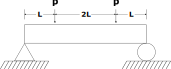
\includegraphics[width=0.7\columnwidth]{Figures/q30.png}
        \centering
        \caption{}
    \end{figure}
    Which one of the following transfer functions is best represented by the above Bode magnitude plot?
    \begin{enumerate}
            \item $\frac{2s}{\brak{1+0.5s}\brak{1+0.25s}^{2}}$
            \item $\frac{4\brak{1+0.5s}}{s\brak{1+0.25s}}$
            \item $\frac{2s}{\brak{1+2s}\brak{1+4s}}$
            \item $\frac{4s}{\brak{1+2s}\brak{1+4s}^{2}}$    \end{enumerate}

    \hfill{\brak{\text{GATE EE 2016}}}

    \item Consider the following state-space representation of a linear time-invariant system.
    $\dot{\mathbf{x}}\brak{t} = \myvec{1 & 0 \\ 0 & 2}\mathbf{x}\brak{t}, y\brak{t}= \mathbf{c}^T\mathbf{x}\brak{t}, \mathbf{c} = \myvec{1 \\ 1}$ and $\mathbf{x}\brak{0} = \myvec{1 \\ 1}$.
    The value of $y\brak{t}$ for $t = \log_e 2$ is \underline{\hspace{2cm}}.

    \hfill{\brak{\text{GATE EE 2016}}}

    \item Loop transfer function of a feedback system is $G\brak{s}H\brak{s} = \frac{s+3}{s^2\brak{s-3}}$. Take the Nyquist contour in the clockwise direction. Then, the Nyquist plot of $G\brak{s}H\brak{s}$ encircles $-1+j0$
    \begin{enumerate}
        \begin{multicols}{2}
            \item once in clockwise direction
            \item twice in clockwise direction
            \item once in anticlockwise direction
            \item twice in anticlockwise direction
        \end{multicols}
    \end{enumerate}

    \hfill{\brak{\text{GATE EE 2016}}}

    \item Given the following polynomial equation
    $s^3 + 5.5s^2 + 8.5s + 3 = 0$,
    the number of roots of the polynomial, which have real parts strictly less than $-1$, is \underline{\hspace{2cm}}.

    \hfill{\brak{\text{GATE EE 2016}}}

    \item Suppose $x_1\brak{t}$ and $x_2\brak{t}$ have the Fourier transforms as shown below.
    \begin{figure}[H]
        \includegraphics[width=0.8\columnwidth]{Figures/q34.png}
        \centering
        \caption{}
    \end{figure}
    Which one of the following statements is TRUE?
    \begin{enumerate}
        \item $x_1\brak{t}$ and $x_2\brak{t}$ are complex and $x_1\brak{t}x_2\brak{t}$ is also complex with nonzero imaginary part
        \item $x_1\brak{t}$ and $x_2\brak{t}$ are real and $x_1\brak{t}x_2\brak{t}$ is also real
        \item $x_1\brak{t}$ and $x_2\brak{t}$ are complex but $x_1\brak{t}x_2\brak{t}$ is real
        \item $x_1\brak{t}$ and $x_2\brak{t}$ are imaginary but $x_1\brak{t}x_2\brak{t}$ is real
    \end{enumerate}

    \hfill{\brak{\text{GATE EE 2016}}}

    \item The output of a continuous-time, linear time-invariant system is denoted by $\mathcal{T}\{x\brak{t}\}$ where $x\brak{t}$ is the input signal. A signal $z\brak{t}$ is called eigen-signal of the system T, when $\mathcal{T}\{z\brak{t}\} = \gamma z\brak{t}$, where $\gamma$ is a complex number, in general, and is called an eigenvalue of T. Suppose the impulse response of the system T is real and even. Which of the following statements is TRUE?
    \begin{enumerate}
        \begin{multicols}{2}
            \item $\cos\brak{t}$ is an eigen-signal but $\sin\brak{t}$ is not
            \item $\cos\brak{t}$ and $\sin\brak{t}$ are both eigen-signals but with different eigenvalues
            \item $\sin\brak{t}$ is an eigen-signal but $\cos\brak{t}$ is not
            \item $\cos\brak{t}$ and $\sin\brak{t}$ are both eigen-signals with identical eigenvalues
        \end{multicols}
    \end{enumerate}

    \hfill{\brak{\text{GATE EE 2016}}}

    \item The current state $Q_A Q_B$ of a two JK flip-flop system is $00$. Assume that the clock rise-time is much smaller than the delay of the JK flip-flop. The next state of the system is
    \begin{figure}[H]
        \includegraphics[width=0.5\columnwidth]{Figures/q36.png}
        \centering
        \caption{}
    \end{figure}
    \begin{enumerate}
        \begin{multicols}{2}
            \item $00$
            \item $01$
            \item $11$
            \item $10$
        \end{multicols}
    \end{enumerate}

    \hfill{\brak{\text{GATE EE 2016}}}

    \item A 2-bit flash Analog to Digital Converter \brak{ADC} is given below. The input is $0 \leq V_{IN} \leq 3$ Volts. The expression for the LSB of the output $B_0$ as a Boolean function of $X_2, X_1,$ and $X_0$ is
    \begin{figure}[H]
        \includegraphics[width=0.6\columnwidth]{Figures/q37.png}
        \centering
        \caption{}
    \end{figure}
    \begin{enumerate}
        \begin{multicols}{2}
            \item $X_0[\overline{X_2 \oplus X_1}]$
            \item $\bar{X}_0[\overline{X_2 \oplus X_1}]$
            \item $X_0[X_2 \oplus X_1]$
            \item $\bar{X}_0[X_2 \oplus X_1]$
        \end{multicols}
    \end{enumerate}

    \hfill{\brak{\text{GATE EE 2016}}}

    \item Two electric charges $q$ and $-2q$ are placed at $\brak{0,0}$ and $\brak{6,0}$ on the x-y plane. The equation of the zero equipotential curve in the x-y plane is
    \begin{enumerate}
        \begin{multicols}{2}
            \item $x = -2$
            \item $y = 2$
            \item $x^2 + y^2 = 2$
            \item $\brak{x+2}^2 + y^2 = 16$
        \end{multicols}
    \end{enumerate}

    \hfill{\brak{\text{GATE EE 2016}}}

    \item In the circuit shown, switch S2 has been closed for a long time. At time $t=0$ switch S1 is closed. At $t=0^+$, the rate of change of current through the inductor, in amperes per second, is \underline{\hspace{2cm}}.
    \begin{figure}[H]
        \includegraphics[width=0.5\columnwidth]{Figures/q39.png}
        \centering
        \caption{}
    \end{figure}

    \hfill{\brak{\text{GATE EE 2016}}}

    \item A three-phase cable is supplying $800$ kW and $600$ kVAr to an inductive load. It is intended to supply an additional resistive load of $100$ kW through the same cable without increasing the heat dissipation in the cable, by providing a three-phase bank of capacitors connected in star across the load. Given the line voltage is $3.3$ kV, $50$ Hz, the capacitance per phase of the bank, expressed in microfarads, is \underline{\hspace{2cm}}.

    \hfill{\brak{\text{GATE EE 2016}}}

    \item A $30$ MVA, 3-phase, $50$ Hz, $13.8$ kV, star-connected synchronous generator has positive, negative and zero sequence reactances, $15\%$, $15\%$ and $5\%$ respectively. A reactance \brak{X_n} is connected between the neutral of the generator and ground. A double line to ground fault takes place involving phases 'b' and 'c', with a fault impedance of j$0.1$ p.u. The value of $X_n$ \brak{\text{in p.u.}} that will limit the positive sequence generator current to $4270$ A is \underline{\hspace{2cm}}.

    \hfill{\brak{\text{GATE EE 2016}}}

    \item If the star side of the star-delta transformer shown in the figure is excited by a negative sequence voltage, then
    \begin{figure}[H]
        \includegraphics[width=0.4\columnwidth]{Figures/q42.png}
        \centering
        \caption{}
    \end{figure}
    \begin{enumerate}
        \begin{multicols}{2}
            \item $V_{AB}$ leads $V_{ab}$ by $60\degree$
            \item $V_{AB}$ lags $V_{ab}$ by $60\degree$
            \item $V_{AB}$ leads $V_{ab}$ by $30\degree$
            \item $V_{AB}$ lags $V_{ab}$ by $30\degree$
        \end{multicols}
    \end{enumerate}

    \hfill{\brak{\text{GATE EE 2016}}}

    \item A single-phase thyristor-bridge rectifier is fed from a $230$ V, $50$ Hz, single-phase AC mains. If it is delivering a constant DC current of $10$ A, at firing angle of $30\degree$, then value of the power factor at AC mains is
    \begin{enumerate}
        \begin{multicols}{2}
            \item $0.87$
            \item $0.9$
            \item $0.78$
            \item $0.45$
        \end{multicols}
    \end{enumerate}

    \hfill{\brak{\text{GATE EE 2016}}}

    \item The switches T1 and T2 in Figure \brak{\text{a}} are switched in a complementary fashion with sinusoidal pulse width modulation technique. The modulating voltage $v_m\brak{t} = 0.8 \sin \brak{200\pi t}$ V and the triangular carrier voltage \brak{v_c} are as shown in Figure \brak{\text{b}}. The carrier frequency is $5$ kHz. The peak value of the $100$ Hz component of the load current \brak{i_L}, in ampere, is \underline{\hspace{2cm}}.
    \begin{figure}[H]
        \includegraphics[width=0.8\columnwidth]{Figures/q44.png}
        \centering
        \caption{}
    \end{figure}

    \hfill{\brak{\text{GATE EE 2016}}}

    \item The voltage \brak{v_s} across and the current \brak{i_s} through a semiconductor switch during a turn-ON transition are shown in figure. The energy dissipated during the turn-ON transition, in mJ, is \underline{\hspace{2cm}}.
    \begin{figure}[H]
        \includegraphics[width=0.6\columnwidth]{Figures/q45.png}
        \centering
        \caption{}
    \end{figure}

    \hfill{\brak{\text{GATE EE 2016}}}

    \item A single-phase $400$ V, $50$ Hz transformer has an iron loss of $5000$ W at the rated condition. When operated at $200$ V, $25$ Hz, the iron loss is $2000$ W. When operated at $416$ V, $52$ Hz, the value of the hysteresis loss divided by the eddy current loss is \underline{\hspace{2cm}}.

    \hfill{\brak{\text{GATE EE 2016}}}

    \item A DC shunt generator delivers $45$ A at a terminal voltage of $220$ V. The armature and the shunt field resistances are $0.01 \ohm$ and $44 \ohm$ respectively. The stray losses are $375$ W. The percentage efficiency of the DC generator is \underline{\hspace{2cm}}.

    \hfill{\brak{\text{GATE EE 2016}}}

    \item A three-phase, $50$ Hz salient-pole synchronous motor has a per-phase direct-axis reactance \brak{X_d} of $0.8$ pu and a per-phase quadrature-axis reactance \brak{X_q} of $0.6$ pu. Resistance of the machine is negligible. It is drawing full-load current at $0.8$ pf \brak{\text{leading}}. When the terminal voltage is $1$ pu, per-phase induced voltage, in pu, is \underline{\hspace{2cm}}.


    \hfill{\brak{\text{GATE EE 2016}}}

    \item A single-phase, $22$ kVA, $2200$ V/ $220$ V, $50$ Hz, distribution transformer is to be connected as an auto-transformer to get an output voltage of $2420$ V. Its maximum kVA rating as an auto transformer is
    \begin{enumerate}
        \begin{multicols}{2}
            \item $22$
            \item $24.2$
            \item $242$
            \item $2420$
        \end{multicols}
    \end{enumerate}

    \hfill{\brak{\text{GATE EE 2016}}}

    \item A single-phase full-bridge voltage source inverter \brak{VSI} is fed from a $300$ V battery. A pulse of $120\degree$ duration is used to trigger the appropriate devices in each half-cycle. The rms value of the fundamental component of the output voltage, in volts, is
    \begin{enumerate}
        \begin{multicols}{2}
            \item $234$
            \item $245$
            \item $300$
            \item $331$
        \end{multicols}
    \end{enumerate}

    \hfill{\brak{\text{GATE EE 2016}}}

    \item A single-phase transmission line has two conductors each of $10$ mm radius. These are fixed at a center-to-center distance of $1$ m in a horizontal plane. This is now converted to a three-phase transmission line by introducing a third conductor of the same radius. This conductor is fixed at an equal distance D from the two single-phase conductors. The three-phase line is fully transposed. The positive sequence inductance per phase of the three-phase system is to be $5\%$ more than that of the inductance per conductor of the single-phase system. The distance D, in meters, is \underline{\hspace{2cm}}.

    \hfill{\brak{\text{GATE EE 2016}}}

    \item In the circuit shown below, the supply voltage is $10 \sin\brak{1000t}$ volts. The peak value of the steady state current through the $1\ohm$ resistor, in amperes, is \underline{\hspace{2cm}}.
    \begin{figure}[H]
        \includegraphics[width=0.6\columnwidth]{Figures/q52.png}
        \centering
        \caption{}
    \end{figure}

    \hfill{\brak{\text{GATE EE 2016}}}

    \item A dc voltage with ripple is given by $v\brak{t} = [100 + 10 \sin\brak{\omega t} - 5 \sin\brak{3\omega t}]$ volts. Measurements of this voltage $v\brak{t}$, made by moving-coil and moving-iron voltmeters, show readings of $V_1$ and $V_2$ respectively. The value of $V_2 - V_1$, in volts, is \underline{\hspace{2cm}}.

    \hfill{\brak{\text{GATE EE 2016}}}

    \item The circuit below is excited by a sinusoidal source. The value of R, in $\ohm$, for which the admittance of the circuit becomes a pure conductance at all frequencies is \underline{\hspace{2cm}}.
    \begin{figure}[H]
        \includegraphics[width=0.5\columnwidth]{Figures/q54.png}
        \centering
        \caption{}
    \end{figure}

    \hfill{\brak{\text{GATE EE 2016}}}

    \item In the circuit shown below, the node voltage $V_A$ is \underline{\hspace{2cm}} V.
    \begin{figure}[H]
        \includegraphics[width=0.6\columnwidth]{Figures/q55.png}
                \centering
        \caption{}
    \end{figure}

    \hfill{\brak{\text{GATE EE 2016}}}

    \item The chairman requested the aggrieved shareholders to \underline{\hspace{2cm}} him.
    \begin{enumerate}
        \begin{multicols}{2}
            \item bare with
            \item bore with
            \item bear with
            \item bare
        \end{multicols}
    \end{enumerate}

    \hfill{\brak{\text{GATE EE 2016}}}

    \item Identify the correct spelling out of the given options:
    \begin{enumerate}
        \begin{multicols}{2}
            \item Managable
            \item Manageable
            \item Mangaeble
            \item Managible
        \end{multicols}
    \end{enumerate}

    \hfill{\brak{\text{GATE EE 2016}}}

    \item Pick the odd one out in the following:
    $13, 23, 33, 43, 53$
    \begin{enumerate}
        \begin{multicols}{2}
            \item $23$
            \item $33$
            \item $43$
            \item $53$
        \end{multicols}
    \end{enumerate}

    \hfill{\brak{\text{GATE EE 2016}}}

    \item R2D2 is a robot. R2D2 can repair aeroplanes. No other robot can repair aeroplanes.
    Which of the following can be logically inferred from the above statements?
    \begin{enumerate}
        \item R2D2 is a robot which can only repair aeroplanes.
        \item R2D2 is the only robot which can repair aeroplanes.
        \item R2D2 is a robot which can repair only aeroplanes.
        \item Only R2D2 is a robot.
    \end{enumerate}

    \hfill{\brak{\text{GATE EE 2016}}}

    \item If $\abs{9y-6} = 3$, then $y^2 - 4y/3$ is \underline{\hspace{2cm}}.
    \begin{enumerate}
        \begin{multicols}{2}
            \item $0$
            \item $+1/3$
            \item $-1/3$
            \item undefined
        \end{multicols}
    \end{enumerate}

    \hfill{\brak{\text{GATE EE 2016}}}

    \item The following graph represents the installed capacity for cement production \brak{in tonnes} and the actual production \brak{in tonnes} of nine cement plants of a cement company. Capacity utilization of a plant is defined as ratio of actual production of cement to installed capacity. A plant with installed capacity of at least $200$ tonnes is called a large plant and a plant with lesser capacity is called a small plant. The difference between total production of large plants and small plants, in tonnes is \underline{\hspace{2cm}}.
    \begin{figure}[H]
        \includegraphics[width=0.7\columnwidth]{Figures/2q6.png}
        \centering
        \caption{}
        
    \end{figure}

    \hfill{\brak{\text{GATE EE 2016}}}

    \item A poll of students appearing for masters in engineering indicated that $60\%$ of the students believed that mechanical engineering is a profession unsuitable for women. A research study on women with masters or higher degrees in mechanical engineering found that $99\%$ of such women were successful in their professions.
    Which of the following can be logically inferred from the above paragraph?
    \begin{enumerate}
        \item Many students have misconceptions regarding various engineering disciplines.
        \item Men with advanced degrees in mechanical engineering believe women are well suited to be mechanical engineers.
        \item Mechanical engineering is a profession well suited for women with masters or higher degrees in mechanical engineering.
        \item The number of women pursuing higher degrees in mechanical engineering is small.
    \end{enumerate}

    \hfill{\brak{\text{GATE EE 2016}}}

    \item Sourya committee had proposed the establishment of Sourya Institutes of Technology \brak{SITs} in line with Indian Institutes of Technology \brak{IITs} to cater to the technological and industrial needs of a developing country.
    Which of the following can be logically inferred from the above sentence?
    Based on the proposal,
    \begin{enumerate}
        \item[\brak{i}] In the initial years, SIT students will get degrees from IIT.
        \item[\brak{ii}] SITs will have a distinct national objective.
        \item[\brak{iii}] SIT like institutions can only be established in consultation with IIT.
        \item[\brak{iv}] SITs will serve technological needs of a developing country.
    \end{enumerate}
    \begin{enumerate}
        \begin{multicols}{2}
            \item \brak{iii} and \brak{iv} only.
            \item \brak{i} and \brak{iv} only.
            \item \brak{ii} and \brak{iv} only.
            \item \brak{ii} and \brak{iii} only.
        \end{multicols}
    \end{enumerate}

    \hfill{\brak{\text{GATE EE 2016}}}

    \item Shaquille O' Neal is a $60\%$ career free throw shooter, meaning that he successfully makes $60$ free throws out of $100$ attempts on average. What is the probability that he will successfully make exactly $6$ free throws in $10$ attempts?
    \begin{enumerate}
        \begin{multicols}{2}
            \item $0.2508$
            \item $0.2816$
            \item $0.2934$
            \item $0.6000$
        \end{multicols}
    \end{enumerate}

    \hfill{\brak{\text{GATE EE 2016}}}

    \item The numeral in the units position of $211^{870} + 146^{127} \times 3^{424}$ is \underline{\hspace{2cm}}.

    \hfill{\brak{\text{GATE EE 2016}}}

    \item The output expression for the Karnaugh map shown below is
    \begin{figure}[H]
        \includegraphics[width=0.4\columnwidth]{Figures/2q1.png}
        \centering
        \caption{}
    \end{figure}
    \begin{enumerate}
        \begin{multicols}{2}
            \item $A + \bar{B}$
            \item $A + \bar{C}$
            \item $\bar{A} + \bar{C}$
            \item $\bar{A} + C$
        \end{multicols}
    \end{enumerate}

    \hfill{\brak{\text{GATE EE 2016}}}

    \item The circuit shown below is an example of a
    \begin{figure}[H]
        \includegraphics[width=0.4\columnwidth]{Figures/2q2.png}
        \centering
        \caption{}
    \end{figure}
    \begin{enumerate}
        \begin{multicols}{2}
            \item low pass filter.
            \item band pass filter.
            \item high pass filter.
            \item notch filter.
        \end{multicols}
    \end{enumerate}

    \hfill{\brak{\text{GATE EE 2016}}}

    \item The following figure shows the connection of an ideal transformer with primary to secondary turns ratio of $1:100$. The applied primary voltage is $100$ V \brak{rms}, $50$ Hz, AC. The rms value of the current I, in ampere, is \underline{\hspace{2cm}}.
    \begin{figure}[H]
        \includegraphics[width=0.4\columnwidth]{Figures/2q3.png}
        \centering
        \caption{}
    \end{figure}

    \hfill{\brak{\text{GATE EE 2016}}}

    \item Consider a causal LTI system characterized by differential equation $\frac{dy\brak{t}}{dt} + \frac{1}{6}y\brak{t} = 3x\brak{t}$. The response of the system to the input $x\brak{t} = 3e^{-t/3}u\brak{t}$, where u\brak{t} denotes the unit step function, is
    \begin{enumerate}
        \item $9e^{-t/3}u\brak{t}$.
        \item $9e^{-t/6}u\brak{t}$.
        \item $9e^{-t/3}u\brak{t} - 6e^{-t/6}u\brak{t}$.
        \item $54e^{-t/6}u\brak{t} - 54e^{-t/3}u\brak{t}$.
    \end{enumerate}

    \hfill{\brak{\text{GATE EE 2016}}}

    \item Suppose the maximum frequency in a band-limited signal $x\brak{t}$ is $5$ kHz. Then, the maximum frequency in $x\brak{t}\cos\brak{2000\pi t}$, in kHz, is \underline{\hspace{2cm}}.

    \hfill{\brak{\text{GATE EE 2016}}}

    \item Consider the function $f\brak{z} = z + z^*$ where $z$ is a complex variable and $z^*$ denotes its complex conjugate. Which one of the following is TRUE?
    \begin{enumerate}
        \item $f\brak{z}$ is both continuous and analytic
        \item $f\brak{z}$ is continuous but not analytic
        \item $f\brak{z}$ is not continuous but is analytic
        \item $f\brak{z}$ is neither continuous nor analytic
    \end{enumerate}

    \hfill{\brak{\text{GATE EE 2016}}}

    \item A $3 \times 3$ matrix $P$ is such that, $P^3=P$. Then the eigenvalues of $P$ are
    \begin{enumerate}
        \begin{multicols}{2}
            \item $1, 1, -1$
            \item $1, 0.5 + j0.866, 0.5 - j0.866$
            \item $1, -0.5 + j0.866, -0.5 - j0.866$
            \item $0, 1, -1$
        \end{multicols}
    \end{enumerate}

    \hfill{\brak{\text{GATE EE 2016}}}

    \item The solution of the differential equation, for $t>0$, $y''\brak{t} + 2y'\brak{t} + y\brak{t} = 0$ with initial conditions $y\brak{0}=0$ and $y'\brak{0}=1$, is \brak{u\brak{t} denotes the unit step function},
    \begin{enumerate}
        \begin{multicols}{2}
            \item $t e^{-t} u\brak{t}$
            \item $\brak{e^{-t} - t e^{-t}}u\brak{t}$
            \item $\brak{-e^{-t} + t e^{-t}}u\brak{t}$
            \item $e^{-t}u\brak{t}$
        \end{multicols}
    \end{enumerate}

    \hfill{\brak{\text{GATE EE 2016}}}

    \item The value of the line integral $\int_C \brak{2xy^2 dx + 2x^2y dy + dz}$ along a path joining the origin $\brak{0,0,0}$ and the point $\brak{1,1,1}$ is
    \begin{enumerate}
        \begin{multicols}{2}
            \item $0$
            \item $2$
            \item $4$
            \item $6$
        \end{multicols}
    \end{enumerate}

    \hfill{\brak{\text{GATE EE 2016}}}

    \item Let f\brak{x} be a real, periodic function satisfying $f\brak{-x} = -f\brak{x}$. The general form of its Fourier series representation would be
    \begin{enumerate}
        \item $f\brak{x} = a_0 + \sum_{k=1}^{\infty} a_k \cos\brak{kx}$
        \item $f\brak{x} = \sum_{k=1}^{\infty} b_k \sin\brak{kx}$
        \item $f\brak{x} = a_0 + \sum_{k=1}^{\infty} a_{2k} \cos\brak{kx}$
        \item $f\brak{x} = \sum_{k=0}^{\infty} a_{2k+1} \sin\brak{\brak{2k+1}x}$
    \end{enumerate}

    \hfill{\brak{\text{GATE EE 2016}}}

    \item A resistance and a coil are connected in series and supplied from a single phase, $100$ V, $50$ Hz ac source as shown in the figure below. The rms values of plausible voltages across the resistance ({$V_R$}) and coil ($V_C$ respectively, in volts, are)
    \begin{figure}[H]
        \includegraphics[width=0.4\columnwidth]{Figures/2q11.png}
        \centering
        \caption{}
    \end{figure}
    \begin{enumerate}
        \begin{multicols}{2}
            \item $65, 35$
            \item $50, 50$
            \item $60, 90$
            \item $60, 80$
        \end{multicols}
    \end{enumerate}

    \hfill{\brak{\text{GATE EE 2016}}}

    \item The voltage \brak{V} and current \brak{A} across a load are as follows.
    $v\brak{t} = 100\sin\brak{\omega t}$, $i\brak{t} = 10\sin\brak{\omega t - 60\degree} + 2\sin\brak{3\omega t} + 5\sin\brak{5\omega t}$.
    The average power consumed by the load, in W, is \underline{\hspace{2cm}}.

    \hfill{\brak{\text{GATE EE 2016}}}

    \item A power system with two generators is shown in the figure below. The system (generators, buses and transmission lines) is protected by six overcurrent relays R1 to R6. Assuming a mix of directional and nondirectional relays at appropriate locations, the remote backup relays for R4 are
    \begin{figure}[H]
        \includegraphics[width=0.4\columnwidth]{Figures/2q13.png}
        \centering
        \caption{}
    \end{figure}
    \begin{enumerate}
        \begin{multicols}{2}
            \item R1, R2
            \item R2, R6
            \item R2, R5
            \item R1, R6
        \end{multicols}
    \end{enumerate}

    \hfill{\brak{\text{GATE EE 2016}}}

    \item A power system has $100$ buses including $10$ generator buses. For the load flow analysis using Newton-Raphson method in polar coordinates, the size of the Jacobian is
    \begin{enumerate}
        \begin{multicols}{2}
            \item $189 \times 189$
            \item $100 \times 100$
            \item $90 \times 90$
            \item $180 \times 180$
        \end{multicols}
    \end{enumerate}

    \hfill{\brak{\text{GATE EE 2016}}}

    \item The inductance and capacitance of a $400$ kV, three-phase, $50$ Hz lossless transmission line are $1.6$ mH/km/phase and $10$ nF/km/phase respectively. The sending end voltage is maintained at $400$ kV. To maintain a voltage of $400$ kV at the receiving end, when the line is delivering $300$ MW load, the shunt compensation required is
    \begin{enumerate}
        \item capacitive
        \item inductive
        \item resistive
        \item zero
    \end{enumerate}

    \hfill{\brak{\text{GATE EE 2016}}}

    \item A parallel plate capacitor filled with two dielectrics is shown in the figure below. If the electric field in the region A is $4$ kV/cm, the electric field in the region B, in kV/cm, is
    \begin{figure}[H]
        \includegraphics[width=0.4\columnwidth]{Figures/2q16.png}
        \centering
        \caption{}
    \end{figure}
    \begin{enumerate}
        \begin{multicols}{2}
            \item $1$
            \item $2$
            \item $4$
            \item $16$
        \end{multicols}
    \end{enumerate}

    \hfill{\brak{\text{GATE EE 2016}}}

    \item A $50$ MVA, $10$ kV, $50$ Hz, star-connected, unloaded three-phase alternator has a synchronous reactance of $1$ p.u. and a sub-transient reactance of $0.2$ p.u. If a 3-phase short circuit occurs close to the generator terminals, the ratio of initial and final values of the sinusoidal component of the short circuit current is \underline{\hspace{2cm}}.

    \hfill{\brak{\text{GATE EE 2016}}}

    \item Consider a linear time-invariant system with transfer function $H\brak{s} = \frac{1}{s+1}$. If the input is $\cos\brak{t}$ and the steady state output is $A \cos\brak{t+\alpha}$, then the value of $A$ is \underline{\hspace{2cm}}.

    \hfill{\brak{\text{GATE EE 2016}}}

    \item A three-phase diode bridge rectifier is feeding a constant DC current of $100$ A to a highly inductive load. If three-phase, $415$ V, $50$ Hz AC source is supplying to this bridge rectifier then the rms value of the current in each diode, in ampere, is \underline{\hspace{2cm}}.

    \hfill{\brak{\text{GATE EE 2016}}}

    \item A buck-boost DC-DC converter, shown in the figure below, is used to convert $24 \, V$ battery voltage 
to $36 \, V$ DC voltage to feed a load of $72 \, W$. It is operated at $20 \, kHz$ with an inductor of $2 \, mH$ and 
output capacitor of $1000 \, \mu F$. All devices are considered to be ideal. The peak voltage across the 
solid-state switch (S), in volt, is \underline{\hspace{2cm}}.
    \begin{figure}[H]
        \includegraphics[width=0.6\columnwidth]{Figures/2q20.png}
        \centering
        \caption{}
    \end{figure}

    \hfill{\brak{\text{GATE EE 2016}}}

    \item For the network shown in the figure below, the frequency \brak{in rad/s} at which the maximum phase lag occurs is, \underline{\hspace{2cm}}.
    \begin{figure}[H]
        \includegraphics[width=0.3\columnwidth]{Figures/2q21.png}
        \centering
        \caption{}
    \end{figure}

    \hfill{\brak{\text{GATE EE 2016}}}

    \item The direction of rotation of a single-phase capacitor run induction motor is reversed by
    \begin{enumerate}
        \item interchanging the terminals of the AC supply.
        \item interchanging the terminals of the capacitor.
        \item interchanging the terminals of the auxiliary winding.
        \item interchanging the terminals of both the windings.
    \end{enumerate}

    \hfill{\brak{\text{GATE EE 2016}}}

    \item In the circuit shown below, the voltage and current sources are ideal. The voltage $V_{out}$ across the current source, in volts, is
    \begin{figure}[H]
        \includegraphics[width=0.4\columnwidth]{Figures/2q23.png}
        \centering
        \caption{}
    \end{figure}
    \begin{enumerate}
        \begin{multicols}{2}
            \item $0$
            \item $5$
            \item $10$
            \item $20$
        \end{multicols}
    \end{enumerate}

    \hfill{\brak{\text{GATE EE 2016}}}

    \item The graph associated with an electrical network has $7$ branches and $5$ nodes. The number of independent KCL equations and the number of independent KVL equations, respectively, are
    \begin{enumerate}
        \begin{multicols}{2}
            \item $2$ and $5$
            \item $5$ and $2$
            \item $3$ and $4$
            \item $4$ and $3$
        \end{multicols}
    \end{enumerate}

    \hfill{\brak{\text{GATE EE 2016}}}

    \item Two electrodes, whose cross-sectional view is shown in the figure below, are at the same potential. The maximum electric field will be at the point
    \begin{figure}[H]
        \includegraphics[width=0.4\columnwidth]{Figures/2q25.png}
        \centering
        \caption{}
    \end{figure}
    \begin{enumerate}
        \item A
        \item B
        \item C
        \item D
    \end{enumerate}

    \hfill{\brak{\text{GATE EE 2016}}}

    \item The Boolean expression $\overline{\brak{\overline{a} + \overline{b} + c + \overline{d}} + \brak{b+\overline{c}}}$ simplifies to
    \begin{enumerate}
        \begin{multicols}{2}
            \item $1$
            \item $\overline{a.b}$
            \item $a.b$
            \item $0$
        \end{multicols}
    \end{enumerate}

    \hfill{\brak{\text{GATE EE 2016}}}

    \item For the circuit shown below, taking the opamp as ideal, the output voltage $V_{out}$ in terms of the input voltages $V_1, V_2$ and $V_3$ is
    \begin{figure}[H]
        \includegraphics[width=0.4\columnwidth]{Figures/2q27.png}
        \centering
        \caption{}
    \end{figure}
    \begin{enumerate}
        \begin{multicols}{2}
            \item $1.8V_1 + 7.2V_2 - V_3$
            \item $2V_1 + 8V_2 - 9V_3$
            \item $7.2V_1 + 1.8V_2 - V_3$
            \item $8V_1 + 2V_2 - 9V_3$
        \end{multicols}
    \end{enumerate}

    \hfill{\brak{\text{GATE EE 2016}}}

    \item Let $x_1\brak{t} \leftrightarrow X_1\brak{\omega}$ and $x_2\brak{t} \leftrightarrow X_2\brak{\omega}$ be two signals whose Fourier Transforms are as shown in the figure below. In the figure, $h\brak{t} = e^{-2|t|}$ denotes the impulse response. For the system shown above, the minimum sampling rate required to sample y\brak{t}, so that y\brak{t} can be uniquely reconstructed from its samples, is
    \begin{figure}[H]
        \includegraphics[width=0.4\columnwidth]{Figures/2q28.png}
        \centering
        \caption{}
    \end{figure}
    \begin{enumerate}
        \begin{multicols}{2}
            \item $2B_1$
            \item $2\brak{B_1+B_2}$
            \item $4\brak{B_1+B_2}$
            \item $\infty$
        \end{multicols}
    \end{enumerate}

    \hfill{\brak{\text{GATE EE 2016}}}

    \item The value of the integral $\int_{-\infty}^{\infty} \brak{\frac{\sin\brak{2\pi t}}{\pi t}}^2 dt$ is equal to
    \begin{enumerate}
        \begin{multicols}{2}
            \item $0$
            \item $0.5$
            \item $1$
            \item $2$
        \end{multicols}
    \end{enumerate}

    \hfill{\brak{\text{GATE EE 2016}}}

    \item Let $y\brak{x}$ be the solution of the differential equation $\frac{d^2y}{dx^2} - 4\frac{dy}{dx} + 4y = 0$ with initial conditions $y\brak{0}=0$ and $\left. \frac{dy}{dx} \right|_{x=0} = 1$. Then the value of $y\brak{1}$ is \underline{\hspace{2cm}}.

    \hfill{\brak{\text{GATE EE 2016}}}

    \item The line integral of the vector field $F = 5xz\hat{i} + \brak{3x^2 + 2y}\hat{j} + x^2z\hat{k}$ along a path from $\brak{0,0,0}$ to $\brak{1,1,1}$ parametrized by $\brak{t, t^2, t}$ is \underline{\hspace{2cm}}.

    \hfill{\brak{\text{GATE EE 2016}}}

    \item Let $P = \myvec{3 & 1 \\ 1 & 3}$. Consider the set S of all vectors $\myvec{x \\ y}$ such that $a^2+b^2=1$ where $\myvec{a \\ b} = P\myvec{x \\ y}$. Then S is
    \begin{enumerate}
        \item a circle of radius $\sqrt{10}$
        \item a circle of radius $\frac{1}{\sqrt{10}}$
        \item an ellipse with major axis along $\myvec{1 \\ 1}$
        \item an ellipse with minor axis along $\myvec{1 \\ 1}$
    \end{enumerate}

    \hfill{\brak{\text{GATE EE 2016}}}

    \item Let the probability density function of a random variable, X, be given as: $f_X\brak{x} = 32e^{-3x}u\brak{x} + ae^{4x}u\brak{-x}$ where $u\brak{x}$ is the unit step function. Then the value of 'a' and $Prob\{X \geq 0\}$, respectively, are
    \begin{enumerate}
        \begin{multicols}{2}
            \item $2, \frac{1}{2}$
            \item $4, \frac{1}{2}$
            \item $2, \frac{1}{4}$
            \item $4, \frac{1}{4}$
        \end{multicols}
    \end{enumerate}

    \hfill{\brak{\text{GATE EE 2016}}}

    \item The driving point input impedance seen from the source $V_s$ of the circuit shown below, in $\ohm$, is \underline{\hspace{2cm}}.
    \begin{figure}[H]
        \includegraphics[width=0.4\columnwidth]{Figures/2q34.png}
        \centering
        \caption{}
    \end{figure}

    \hfill{\brak{\text{GATE EE 2016}}}

    \item The z-parameters of the two port network shown in the figure are $z_{11} = 40\ohm$, $z_{12} = 60\ohm$, $z_{21} = 80\ohm$ and $z_{22} = 100\ohm$. The average power delivered to $R_L=20\ohm$, in watts, is \underline{\hspace{2cm}}.
    \begin{figure}[H]
        \includegraphics[width=0.6\columnwidth]{Figures/2q36.png}
        \centering
        \caption{}
    \end{figure}

    \hfill{\brak{\text{GATE EE 2016}}}

    \item In the balanced 3-phase, $50$ Hz, circuit shown below, the value of inductance \brak{L} is $10$ mH. The value of the capacitance \brak{C} for which all the line currents are zero, in millifarads, is \underline{\hspace{2cm}}.
    \begin{figure}[H]
        \includegraphics[width=0.4\columnwidth]{Figures/2q35.png}
        \centering
        \caption{}
    \end{figure}

    \hfill{\brak{\text{GATE EE 2016}}}

    \item In the circuit shown below, the initial capacitor voltage is $4\,\text{V}$. 
Switch $S_1$ is closed at $t=0$. The charge (in $\mu\text{C}$) lost by the
capacitor from $t=25\,\mu\text{s}$ to $t=100\,\mu\text{s}$ is
\underline{\hspace{2cm}}.
    \begin{figure}[H]
        \includegraphics[width=0.4\columnwidth]{Figures/2q37.png}
        \centering
        \caption{}
    \end{figure}

    \hfill{\brak{\text{GATE EE 2016}}}

    \item The single line diagram of a balanced power system is shown in the figure. The voltage magnitude at the generator internal bus is constant and $1.0$ p.u. The p.u. reactances of different components in the system are also shown in the figure. The infinite bus voltage magnitude is $1.0$ p.u. A three phase fault occurs at the middle of line 2. The ratio of the maximum real power that can be transferred during the pre-fault condition to the maximum real power that can be transferred under the faulted condition is \underline{\hspace{2cm}}.
    \begin{figure}[H]
        \includegraphics[width=0.4\columnwidth]{Figures/2q38.png}
        \centering
        \caption{}
    \end{figure}


    \hfill{\brak{\text{GATE EE 2016}}}

    \item The open loop transfer function of a unity feedback control system is given by \\
    \begin{center}
        
   $G\brak{s} = \frac{K\brak{s+1}}{s\brak{1+Ts}\brak{1+2s}}, K>0, T>0$.\\
    \end{center}  The closed loop system will be stable if,
    \begin{enumerate}
        \begin{multicols}{2}
            \item $0 < T < \frac{4\brak{K+1}}{K-1}$
            \item $0 < K < \frac{4\brak{T+2}}{T-2}$
            \item $0 < K < \frac{T+2}{T-2}$
            \item $0 < T < \frac{8\brak{K+1}}{K-1}$
        \end{multicols}
    \end{enumerate}

    \hfill{\brak{\text{GATE EE 2016}}}

    \item At no load condition, a 3-phase, $50$ Hz, lossless power transmission line has sending-end and receiving-end voltages of $400$ kV and $420$ kV respectively. Assuming the velocity of traveling wave to be the velocity of light, the length of the line, in km, is \underline{\hspace{2cm}}.

    \hfill{\brak{\text{GATE EE 2016}}}

    \item The power consumption of an industry is $500$ kVA, at $0.8$ p.f. lagging. A synchronous motor is added to raise the power factor of the industry to unity. If the power intake of the motor is $100$ kW, the p.f. of the motor is \underline{\hspace{2cm}}.

    \hfill{\brak{\text{GATE EE 2016}}}

    \item The flux linkage ($\lambda$) and current (i) relation for an electromagnetic system is $\lambda = (\sqrt{i})/g$. When $i=2$A and $g$ \brak{air-gap length} = $10$ cm, the magnitude of mechanical force on the moving part, in N, is \underline{\hspace{2cm}}.

    \hfill{\brak{\text{GATE EE 2016}}}

    \item The starting line current of a $415$ V, 3-phase, delta connected induction motor is $120$ A, when the rated voltage is applied to its stator winding. The starting line current at a reduced voltage of $110$ V, in ampere, is \underline{\hspace{2cm}}.

    \hfill{\brak{\text{GATE EE 2016}}}

    \item A single-phase, $2$ kVA, $100/200$ V transformer is reconnected as an auto-transformer such that its kVA rating is maximum. The new rating, in kVA, is \underline{\hspace{2cm}}.

    \hfill{\brak{\text{GATE EE 2016}}}

    \item A full-bridge converter supplying an RLE load is shown in figure. The firing angle of the bridge converter is $120\degree$. The supply voltage $v_m\brak{t} = 200\pi \sin\brak{100\pi t}$ V, R=$20\ohm$, E=$800$ V. The inductor L is large enough to make the output current $I_L$ a smooth dc current. Switches are lossless. The real power fed back to the source, in kW, is \underline{\hspace{2cm}}.
    \begin{figure}[H]
        \includegraphics[width=0.6\columnwidth]{Figures/2q45.png}
        \centering
        \caption{}
    \end{figure}

    \hfill{\brak{\text{GATE EE 2016}}}

    \item A three-phase Voltage Source Inverter \brak{VSI} as shown in the figure is feeding a delta connected resistive load of $30 \ohm$/phase. If it is fed from a $600$ V battery, with $180\degree$ conduction of solid-state devices, the power consumed by the load, in kW, is \underline{\hspace{2cm}}.
        \begin{figure}[H]
        \includegraphics[width=0.6\columnwidth]{Figures/2q46.png}
        \centering
        \caption{}
    \end{figure}

    \hfill{\brak{\text{GATE EE 2016}}}

    \item A DC-DC boost converter, as shown in the figure below, is used to boost $360$V to $400$ V, at a power of $4$ kW. All devices are ideal. Considering continuous inductor current, the rms current in the solid state switch \brak{S}, in ampere, is \underline{\hspace{2cm}}.
        \begin{figure}[H]
        \includegraphics[width=0.6\columnwidth]{Figures/2q47.png}
        \centering
        \caption{}
    \end{figure}

    \hfill{\brak{\text{GATE EE 2016}}}

    \item A single-phase bi-directional voltage source converter (VSC) is shown in the figure below. 
All devices are ideal. It is used to charge a battery at $400\,\text{V}$ with power of $5\,\text{kW}$ 
from a source $V_s = 220\,\text{V (rms)}$, $50\,\text{Hz}$ sinusoidal AC mains at unity p.f. 
If its AC-side interfacing inductor is $5\,\text{mH}$ and the switches are operated at $20\,\text{kHz}$, 
then the phase shift $(\delta)$ between AC mains voltage $(V_s)$ and fundamental AC rms VSC voltage $(V_{C1})$, 
in degree, is \underline{\hspace{2cm}}.
\begin{figure}[H]
        \includegraphics[width=0.6\columnwidth]{Figures/2q48.png}
        \centering
        \caption{}
    \end{figure}
    

    \hfill{\brak{\text{GATE EE 2016}}}

    \item Consider a linear time-invariant system $\dot{x}=Ax$, with initial condition $x(0)$ at $t=0$.
Suppose $\alpha$ and $\beta$ are eigenvectors of a $(2\times2)$ matrix $A$ corresponding to
distinct eigenvalues $\lambda_1$ and $\lambda_2$, respectively. Then the response $x(t)$ of the
system due to initial condition $x(0)=\alpha$ is
    \begin{enumerate}
            \item $e^{\lambda_1 t}\alpha$
            \item $e^{\lambda_2 t}\beta$
            \item $e^{\lambda_2 t}\alpha$
            \item $e^{\lambda_1 t}\alpha + e^{\lambda_2 t}\beta$
    \end{enumerate}

    \hfill{\brak{\text{GATE EE 2016}}}

    \item A second-order real system has the following properties:
    a) the damping ratio $\zeta = 0.5$ and undamped natural frequency $\omega_n=10$ rad/s,
    b) the steady state value of the output, to a unit step input, is $1.02$.
    The transfer function of the system is
    \begin{enumerate}
            \item $\frac{1.02}{s^2+5s+100}$
            \item $\frac{102}{s^2+10s+100}$
            \item $\frac{100}{s^2+10s+100}$
            \item $\frac{102}{s^2+5s+100}$
    \end{enumerate}

    \hfill{\brak{\text{GATE EE 2016}}}

    \item Three single-phase transformers are connected to form a delta-star three-phase transformer of $110$ kV/ $11$ kV. The transformer supplies at $11$ kV a load of $8$ MW at $0.8$ p.f. lagging to a nearby plant. Neglect the transformer losses. The ratio of phase currents in delta side to star side is
    \begin{enumerate}
        \begin{multicols}{2}
            \item $1 : 10\sqrt{3}$
            \item $10\sqrt{3} : 1$
            \item $1 : 10$
            \item $\sqrt{3} : 10$
        \end{multicols}
    \end{enumerate}

    \hfill{\brak{\text{GATE EE 2016}}}

    \item The gain at the breakaway point of the root locus of a unity feedback system with open loop transfer function $G\brak{s} = \frac{K}{s\brak{s-1}\brak{s-4}}$ is
    \begin{enumerate}
        \begin{multicols}{2}
            \item $1$
            \item $2$
            \item $5$
            \item $9$
        \end{multicols}
    \end{enumerate}

    \hfill{\brak{\text{GATE EE 2016}}}

    \item Two identical unloaded generators are connected in parallel as shown in the figure. Both the generators are having positive, negative and zero sequence impedances of j$0.4$ p.u., j$0.3$ p.u. and j$0.15$ p.u., respectively. If the pre-fault voltage is $1$ p.u., for a line-to-ground \brak{L-G} fault at the terminals of the generators, the fault current, in p.u., is \underline{\hspace{2cm}}.
    \begin{figure}[H]
        \includegraphics[width=0.6\columnwidth]{Figures/2q53.png}
        \centering
        \caption{}
    \end{figure}

    \hfill{\brak{\text{GATE EE 2016}}}

    \item An energy meter, having meter constant of $1200$ revolutions/kWh, makes $20$ revolutions in $30$ seconds for a constant load. The load, in kW, is \underline{\hspace{2cm}}.

    \hfill{\brak{\text{GATE EE 2016}}}

    \item A rotating conductor of $1$ m length is placed in a radially outward \brak{about the z-axis} magnetic flux density \brak{B} of $1$ Tesla as shown in figure below. Conductor is parallel to and at $1$ m distance from the z-axis. The speed of the conductor in r.p.m. required to induce a voltage of $1$ V across it, should be \underline{\hspace{2cm}}.
\begin{figure}[H]
        \includegraphics[width=0.6\columnwidth]{Figures/2q55.png}
        \centering
        \caption{}
    \end{figure}
    \hfill{\brak{\text{GATE EE 2016}}}

\end{enumerate}

\end{document}